% !Mode:: "TeX:UTF-8"

\chapter{流数据的三维目标检测与跟踪}
\label{methodology}
本章将详细介绍本工作提出的流数据三维目标检测与跟踪框架 \textbf{DODT} (\textbf{D}ual-way \textbf{O}bject \textbf{D}etection and \textbf{T}racking)。本章先介绍DODT的整体网络架构,然后再重点分析各个模块的功能以及实现。

\section{框架整体结构}
\label{total_structure}
\begin{figure}[h]
	%\vspace{-0.3cm}
	\begin{center}
		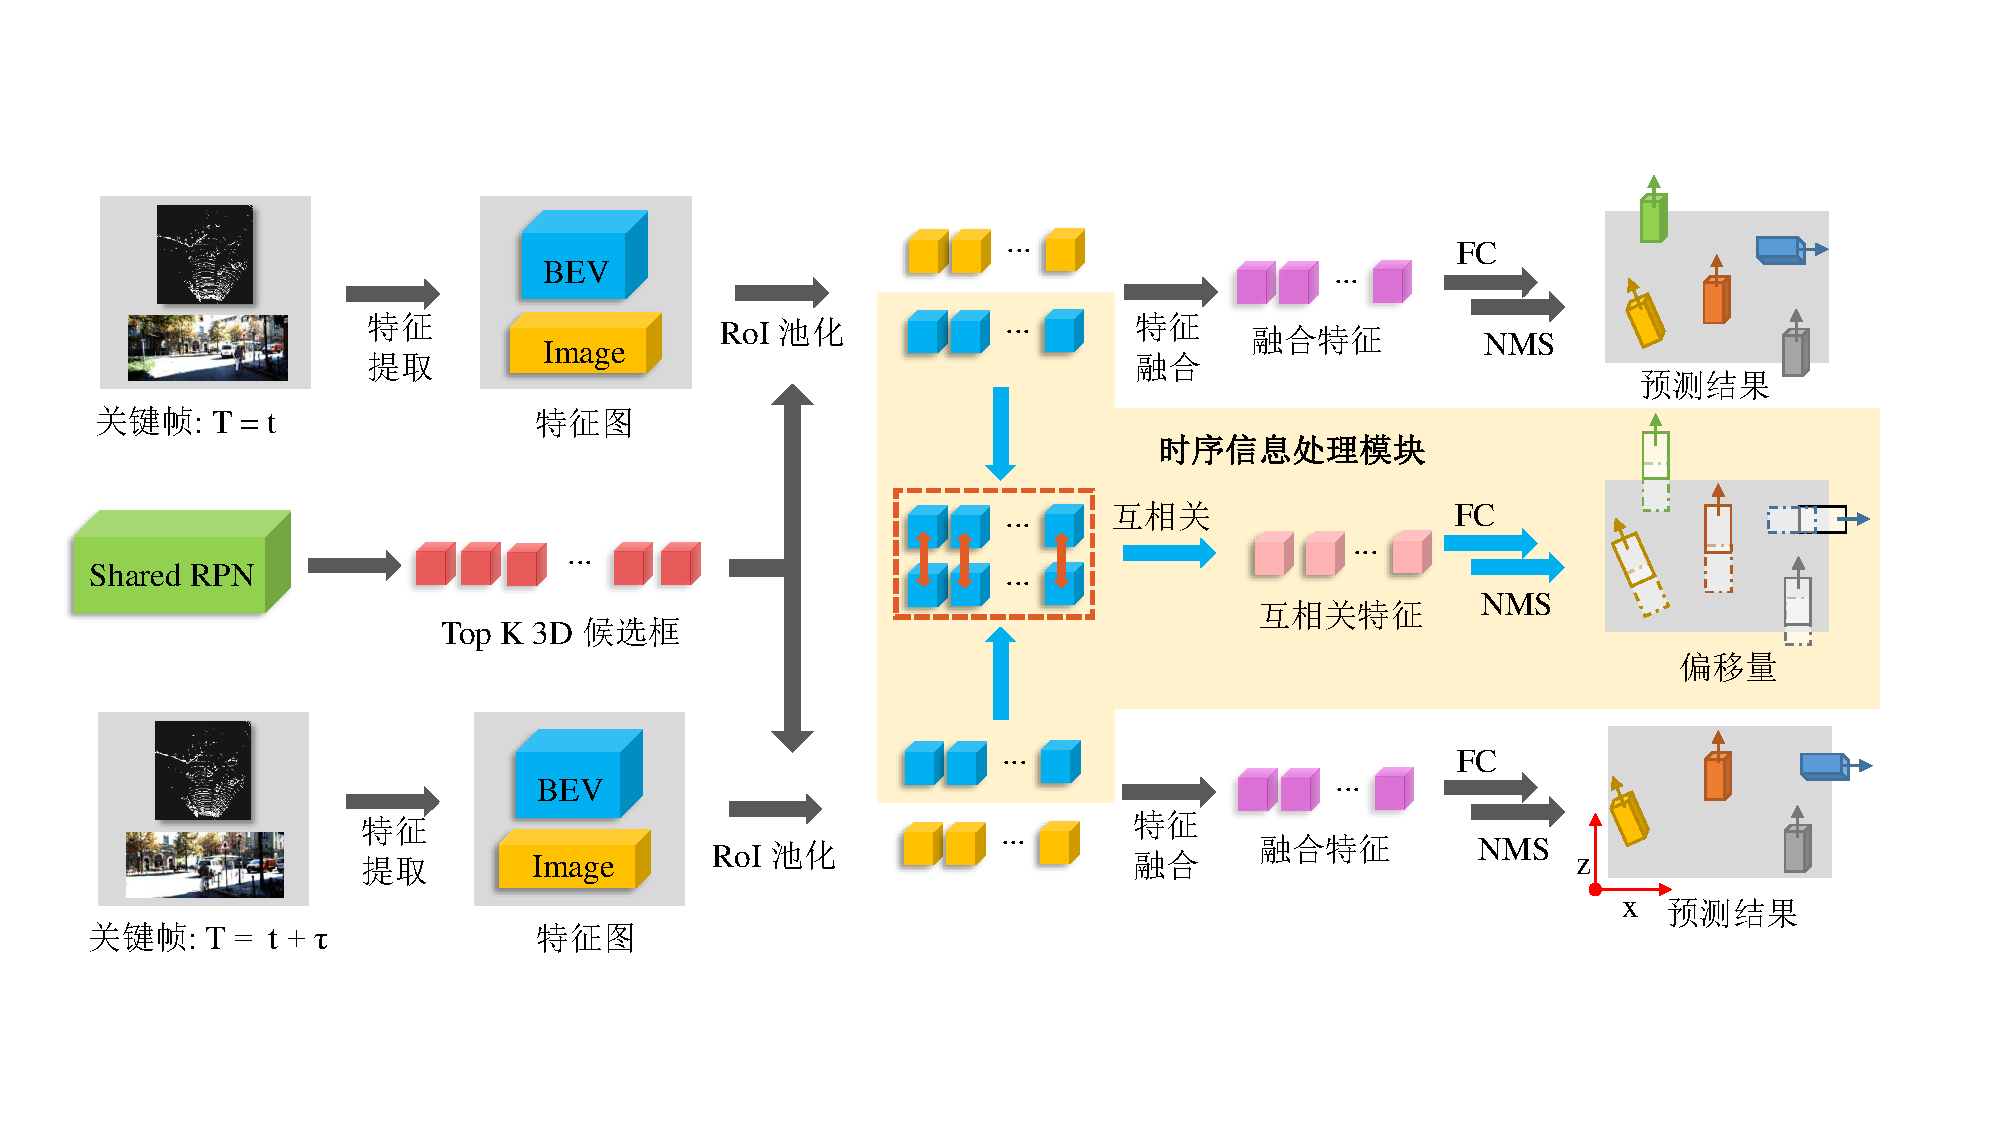
\includegraphics[trim={1.1cm, 2.5cm, 1.5cm, 2.5cm}, clip, width=\textwidth]{imgs/structure_final.pdf}
	\end{center}
	\vspace{-0.8cm}
	\caption{DODT 框架结构,FC表示全连接层,NMS是非极大值抑制过程。}
	\label{fig:dodt}
	%\vspace{-0.3cm}
\end{figure}


DODT网络是双路结构,其结构如\figurename \, \ref{fig:dodt} 所示。DODT由四个小模块组成:三维物体检测模块、Shared RPN模块、时序信息处理模块以及运动插值模块。三维物体检测模块有两个分支,分别负责检测两相邻关键帧中的物体。检测模块的网络结构是基于AVOD\cite{ku2018joint}构建的,为二阶段物体检测框架的三维扩展,该模块的详细结构将在3.2节介绍。Shared RPN 模块负责生成二阶段物体检测中的候选框,与传统RPN不同的是,Shared RPN生成的3D候选框可以被两个三维检测分支共同使用,该模块将在3.3节详细介绍。时序处理模块为 \figurename \, \ref{fig:dodt} 的浅黄色区域,该模块通过对相邻关键帧的点云俯视图(Bird Eye View,BEV)特征匹配块进行相关(correlation) 操作提取帧间的时序信息,然后预测同一物体物体在两关键帧的位置位置偏移。3.4节将详细介绍时序处理模块的实现原理。运动插值模块主要是由独立于网络结构的运动插值算法构成,该算法使用三维物体检测模块对两关键帧的检测结果以及时序处理模块输出的位置偏移信息,将关键帧的检测结果传播到非关键帧,实现流数据的三维物体检测与追踪。该算法的详细流程将会在3.5节重点介绍。


\section{三维物体检测模块}
\label{3d_detection_module}

DODT框架的三维物体检测模块融合了点云与图像信息,预测自动驾驶场景中车辆的三维位姿信息。由于该检测模块是基于AVOD\cite{ku2018joint}网络,为二阶段物体检测模块,因此包含候选框提取网络。由于本框架的候选框提取网络与AVOD有所不同,因此将在下一节详细介绍。本节不展开介绍候选框提取环节。本节将依次介绍数据预处理、特征提取、RoI池化、特征融合以及最终的预测框生成等物体检测中的关键环节。

\subsection{数据预处理}

DODT融合RGB图像数据以及激光雷达数据进行三维物体检测,因此每一帧数据都同时包含图像以及点云。

\subsection{特征提取}

\subsection{RoI 池化}

\subsection{特征融合}

\subsection{预测框生成}

\section{Shared RPN模块}
\label{shared_rpn}

\begin{figure}
	%\vspace{-0.5cm}
	\centering
	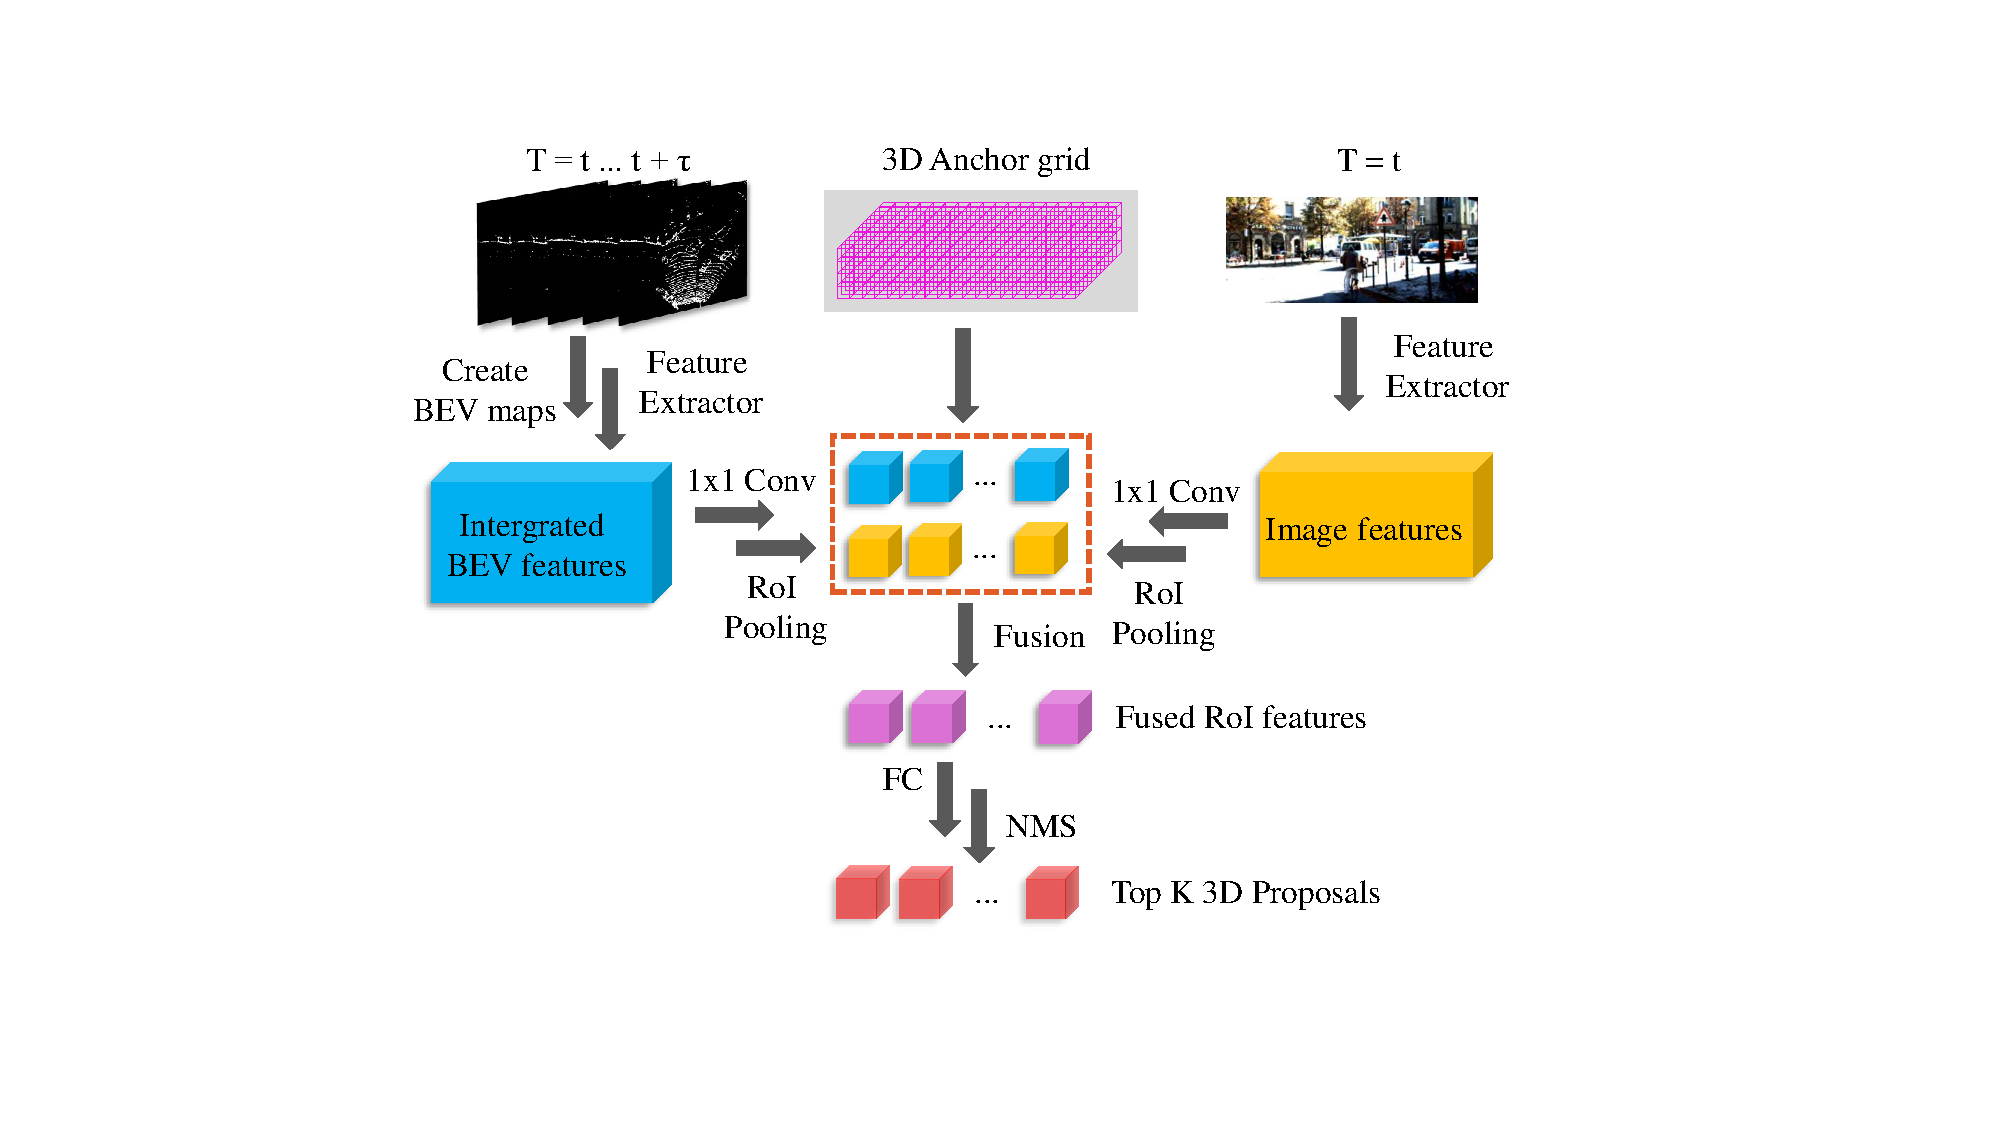
\includegraphics[trim={7cm, 3.5cm, 8cm, 2cm}, clip,width=0.8\textwidth]{imgs/rpn_final.pdf}
	%\vspace{-0.3cm}
	\caption{Shared RPN 模块。}
	\label{fig:shared_rpn}
	%\vspace{-1.5cm}
\end{figure}


\begin{figure}[t]
	\begin{center}
		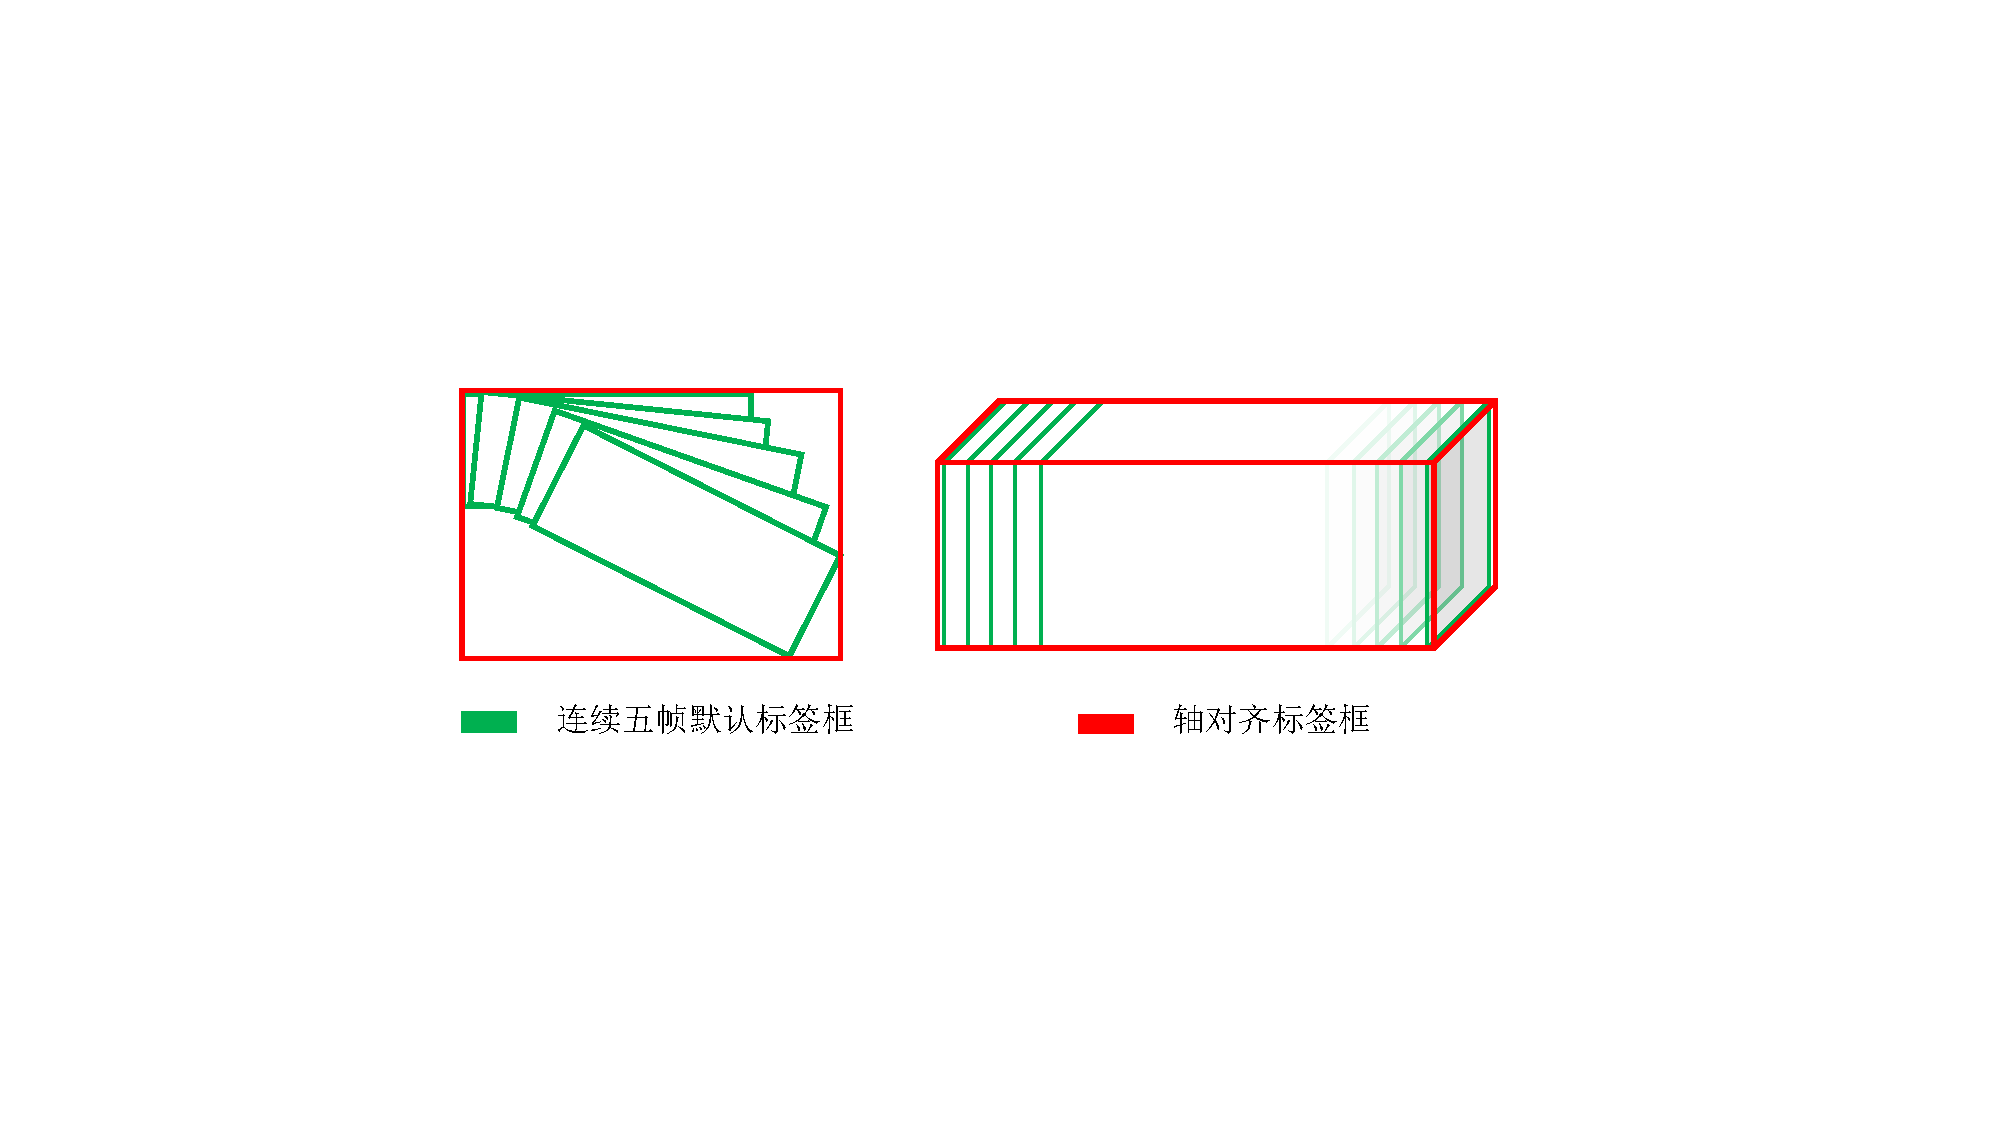
\includegraphics[trim={6cm, 6cm, 8cm, 6cm}, clip, width=0.8\textwidth]{imgs/axis-aligned-boxes.pdf}
	\end{center}
	\vspace{-0.8cm}
	\caption{\textcolor{green}{绿色} 框是五帧中目标的标签框,\textcolor{red}{红色}框是为训练\textit{Shared RPN} 而新生成的共享候选框标签。}
	\label{fig:integrated_boxes}
\end{figure}


\section{时序信息处理模块}
\label{temporal_module}

\begin{equation}
\delta^{t, t+\tau} = \\
\begin{cases}
(\frac{d_{x}^{t+\tau} - d_{x}^{t}}{d^t_{w}}, \frac{d_{z}^{t+\tau} - d_{z}^{t} }{d^t_{l}}, \frac{d_{ry}^{t+\tau} - d_{ry}^{t}}{d^t_{ry}}) & p_{co} = 1.0 \\
(0.0,0.0, 0.0) &  otherwise
\end{cases}
\end{equation}

\section{运动插值模块}
\label{interpolation}

\begin{algorithm}
	\caption{基于运动模型的插值算法(MoI Algorithm)}
	\label{alg:interpolation}
	\textbf{输入: } $D^t= [d^t_0, d^t_1, ..., d^t_{N_t}], D^{t+\tau}= [d^{t+\tau}_0, d^{t+\tau}_1, ..., d^{t+\tau}_{N_{t+\tau}}],$
	$\Delta^{t, t+\tau}=[\delta^{t, t+\tau}_0, \delta^{t, t+\tau}_1, ..., \delta^{t, t+\tau}_{N_{max}}], N_{max} = \max\{N_t, N_{t+\tau}\}$\\
	\textbf{输出: } $D = [D^t, D^{t+1}, ..., D^{t+\tau}]$\\
	\textbf{初始化:} $D_{temp} = D^{t+\tau}, D, p_{co}^{max} = 0.5$ \\
	\For{$d^t_i \emph{ in } D^t$}{
		$\Delta d^{t, t+ \tau}_{i} = (d^t_{i, w} \cdot \delta^{t, t+\tau}_{i,x}, 0, d^t_{i, l} \cdot \delta^{t, t+\tau}_{i,z}, 0, 0, d^t_{i, ry} \cdot \delta^{t, t+\tau}_{i,ry})$
		$d' = getMatched(d^t_i+\Delta d^{t, t+ \tau}_{i}, D_{temp})$\\
		\If{$d'$}{
			$d^{t+1}_i,..., d^{t+\tau-1}_i = Interpolate(d^t_i, d')$\\
			remove $d'$ from $D_{temp}$
		}
		\ElseIf{$p_{co}^i \geq p_{co}^{max}$}{
			$d^{t+1}_i,..., d^{t+\tau}_i = Interpolate(d^t_i, d^t_i + \Delta d^{t, t+ \tau}_{i})$
		}
		\Else{generate $(d^{t+1}_i,..., d^{t+\tau-1}_i)$ by motion model}
	}
	\If{$D_{temp}$ is not empty}{
		\For{$d^{t+\tau}_j \emph{ in } D_{temp}$}{
			\If{$p_{co}^j \geq p_{co}^{max}$}{
				$d^{t}_j,..., d^{t+\tau-1}_j = Interpolate(d^{t+\tau}_j - \Delta d^{t, t+ \tau}_{j}, d^{t+\tau}_j)$
			}
			\Else{
				generate $(d^{t+1}_j,..., d^{t+\tau-1}_j)$ by motion model
			}
		}
	}
\end{algorithm}



\section{多目标追踪}
\label{tracking_module}




\section{本章总结}
\label{metho_conclusion}

% 打印时插入必要的空白页
\ifprint
\newpage
\thispagestyle{empty}
\mbox{}

% 避免空白页影响页码编号
\clearpage
\setcounter{page}{10}
\fi